% ====================================================================
%+
% SECTION:
%    sn.tex
%
% CHAPTER:
%    transients.tex
%
% ELEVATOR PITCH:
%
%-
% ====================================================================

\section{Supernovae as Transients}
\def\secname{\chpname:SNtransients}\label{sec:\secname}

\credit{fedhere}

Supernovae (SNe) represent the final dramatic stages of the life of many
stars. The term SN covers a diverse set of phenomena: explosion of
low mass stars in binary systems, thermonuclear SN or SN Ia (also
discussed in \autoref{sec:supernovae}), explosions of high mass stars,
core collapse (CC) SNe, and even terminal explosions of more exotic
systems, yet to be understood, like Super Luminous SNe
(SLSNe). Phenomenologically, the observables of the explosion are
also diverse. The transient duration ranges from weeks to
months and even years. The electromagnetic energy radiated ranges between
$\sim0.1$ (faintest CC SNe), to $\sim1$ (SN Ia) and $\sim100$ (SLSNe)
$\times 10^{49}$ erg, corresponding to absolute magnitudes at peak
ranging between $\sim-19$ and $\sim-22$.

LSST's contribution to SNe studies can be substantial. Synoptic
surveys such as SDSS, SNLS, PTF, PanSTARRS have revolutionized our
understanding of SN time and again, exposing their diversity,
and revealing different progenitor channels. LSST's first crucial
input will be discovery: the normal type Ia SN rate out to redshift
$z=1$ is estimated to be $\sim200 ~(\mathrm{sq. deg.})^{-1}$ per
year\footnote{\url{http://www.lsst.org/sites/default/files/docs/Wood-Vasey_086.11.pdf}},
and SN~Ia represent only about 1/4 of all SN
events~\citep{Li11b}: tens of millions of stars will explode
within the LSST footprint every year. The main factors affecting
LSST SN science concern:
\begin{enumerate}
\item
LSST's SN discovery power,
\item
LSST's discrimination power,
\item
the quality of the statistical sample over time.
\end{enumerate}
Items 1 and 2 are \emph{time sensitive}, while the latter
is not, although it is interesting to understand the pace at which a
science question can be advanced in the lifetime of LSST.

{\bf \emph{Discovery:}} the SN~Ia discovery is rate is a standard LSST time-domain metric: a
fraction of $\sim40\%$ SN~Ia $z\lesssim0.5$ are expected to be discovered pre-peak
luminosity within the standard LSST survey
(e.g. \opsimdbref{db:baseCadence}~Figure~\ref{fig:enigmaEarlySNe}). The
topic of SNe discovery is discussed in further detail in
\autoref{sec:supernovae}.

The next step is then {\emph{discrimination}}, and the question we need
to answer, for SNe as well as for most other transients, is: will LSST
photometry allow us to distinguish SN from other transients, and to
distinguish the different types of SN? And further: will this be
achievable in time to appropriately direct follow-up efforts? This is
particularly difficult considering that photometric classification
schemes have only achieved modest performances in distinguishing, for
example, SN~Ic from SN~Ia.

When a large statistical sample of SNe is generated, LSST's photometry
may allow setting constraints on the diversity of the sample, even as a
standalone survey, without the aid of follow-up efforts.  {\emph Thus
  LSST \bf{alone} can shed light on the diversity within the
  population of SN}, which in turn may constrain the genesis of the
explosion.\footnote{Reliable typing of a SN and redshift determination
  would still require auxiliary data.} For SN~Ia, where the exploding
star is a carbon-oxygen White Dwarf (WD), a major outstanding question
that can be answered by an LSST photometric sample is
what is the percentage of SN Ia that arise from a
\emph{double-degenerate} (DD) progenitor system (a carbon-oxygen WD-WD
binary), from a \emph {single-degenerate} (SD) system (a WD-Main Sequence
 or WD-Red Giant (RG) binary), or from a \emph{merger} (a WD-WD
 binary with a He and a carbon-oxygen WD).
 Answering this question would reduce the
scatter in the Hubble diagram if SNe from different progenitors are
shown to require different standardization~\citep{Scolnic2014}. On the
CC~SN side: the diversity of SN sub-classes, and the relationship
between them (is there a phenomenological continuum or are they actually
distinct classes, e.g. between IIp and IIL, or Ib and IIb?) is yet to
be understood. Exceptionally well-studied objects may answer these
questions: individual SN Ia with tight constraints on the progenitor
system show, for example, that both single and double degenerate
progenitors exist (e.g. SN 2011fe, \citealt{Li11}, ~\citealt{Olling15}
and PTF 11kx, \citealt{Dilday12}). However, a statistical sample is
needed to set constraints on populations~\citep{Hayden2010, Bianco11}.

Thus the technical question to be answered is: how much detail can be
sacrificed in favor of sample size without compromising diagnostic
power? And the diagnostic power relies on color and sampling: thus
what is the trade-off between cadence in the same filter, and
observations in different filters. Specifically, transients can be
distinguished early from two photometric characteristics: rise time
and color. There is a tension between these observables, as discussed
in Section~\ref{sec:\chpname:transientsAge}. Obtaining colors relies
of course on obtaining photometry in different bands as close as
possible to \emph{simultaneously}.  However, assessing the rise slope
is best done with a single filter, so prompt characterization also
needs multiple epochs within a night, although separated by at least a
few hours, in the same filter, as observing with different
filters it is impossible (or very hard) to separate shape from
color. Colors are an important diagnostic for the
statistical sample: as long as the epoch of peak is reliably assessed
coadded light curves can be studied, which is the goal of the analysis
that follows.

\subsection{Distinguishing progenitor scenarios}

In this chapter we envision and design a SN related metric that works
on a large sample (months-to-years of LSST data) and assesses the
ability to characterize the contribution of SNe with specific features
to the global population: as a test case we will use the identification of
an early blue excess for SN type Ia, a signature of interaction with a
companion, and thus of a SD progenitor. Equivalently, the presence of
an early blue excess in CC~SNe could be the signature of
shock breakout which directly measures the radius of the progenitor
star. We perform the simulation on SN~Ia since statistical studies of
samples that set constraints on progenitor fractions (fraction of DD
vs SD progenitors) exist and can be used as a
benchmark~\citep{Hayden2010, Bianco11}.  What we evaluate as a
\emph{figure of merit} (FoM) for this science deviates from the
guidelines for figures of merit, since LSST will surely be able to
answer this question \emph{at some point} and we measure \emph{how
  fast} LSST can answer this question. Our FoM is time
within the survey required to achieve a sufficiently large sample of
SNe to enable us to distinguish
populations with different contribution from DD and SD progenitors.
We rely on simulations of the observables of the population for
different sample sizes, and on the \MAFmetric{transientAsciiMetric} to
determine the detectability of interacting vs non-interacting
SNe. We are developing a metric (\texttt{colorGapMetric}) to assess
the gap between of detections in 2 filters. In the meantime, we rely on
the estimated of the gap between observations in a single filter, and
in any filters (see~\autoref{sec:\chpname:analysis}).

We simulate interacting SNe from the Nugent templates \citep{Nugent02}
injecting the angle-dependent effects of interaction with a companion
as simulated by \citep{Kasen10}, for a $2~M_\odot$ and a $6~M_\odot$
MS companion stars, and a $1~M_\odot$ RG companion, following the
procedure designed in ~\citep{Bianco11}. We create synthetic progenitor
populations with a fraction of single degenerate progenitor systems
$0.05 \leq f_\mathrm{SD} \leq 0.6 $ in 0.05 intervals, and random lines of
sight with respect to the binary's geometry. One such lightcurve, with
maximal interaction effects, is shown in \autoref{fig:kasenlc}, also
indicating how it may be observed by LSST. For each population, we
simulate the observation of colors by selecting random epochs with a
granularity of 1 day within the first 10 days after explosion, and
subtracting the magnitude in different filters at the same epoch
$\pm~1$~day for each SN, and we include the effects of observational
noise by generating datapoints from a draw within a Gaussian
distribution centered at the color measured in the previous step and
with standard deviation $\sigma_\mathrm{pop} = 0.1$, 0.3, and 0.5.
The SNR requirement is
translated into a requirement on each
observation of $\mathrm{SNR} >
\frac{1.0}{\sqrt{2.0}~\sigma_\mathrm{pop}}$.
We generate populations of $N_\mathrm{pop}=100$,~1000,~10000 $z~=~0.5$ SNe,
observed in $g'-r'$, as a representative case. Because the effect is
heavily chromatic and becomes essentially negligible
by $r$ band, $u'-i'$ gives the most leverage. However $g'$ and $r'$
are the best observed LSST bands in most cadences. An extension of
this work should then consider $g'-r'$, $u'-r'$, $g'-i'$, and $u'-i'$.

\begin{figure}[hbt]
\centerline{
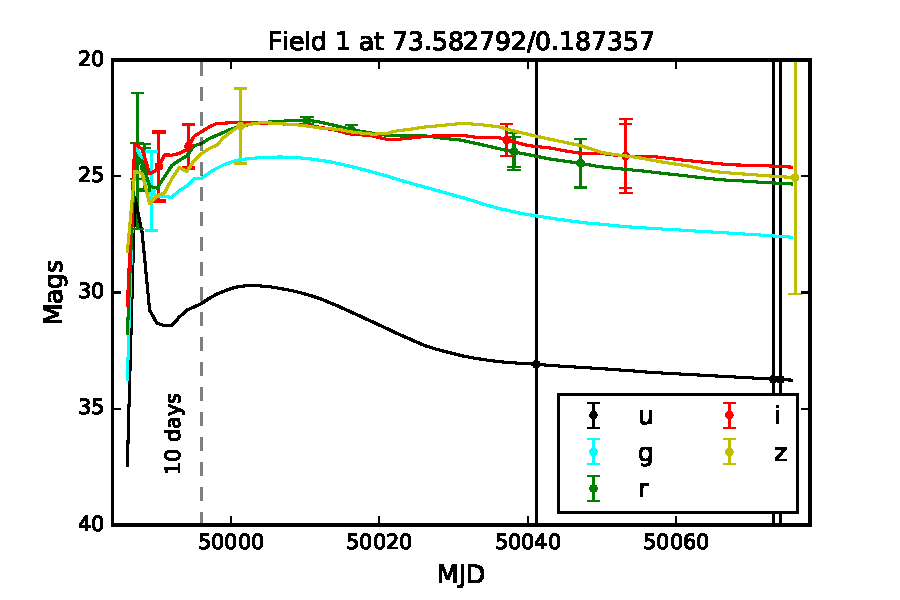
\includegraphics[width=0.6\textwidth]{figs/transients/LSST_Kasen_lcv0.pdf}
}
\caption{ A normal SN Ia lightcure at z=0.5 showing interaction with a
  RG companion as seen from the most favorable viewing angle: the
  effect of interaction as simulated by \citet{Kasen10} is added on
  top of a lightcurve simulated from the \citealt{Nugent02}
  templates. The data points represent one possible set of LSST
  observations of this transient, obtained by running the
  \MAFmetric{transientAsciiMetric}.  This particular event is detected in
  $g'$, $r'$, and $i'$ within the first 10 days.}
\label{fig:kasenlc}
\end{figure}

We perform Kolmogorov-Smirnoff ($KS$) and Anderson-Darling ($AD$) tests
to evaluate our diagnostic power as a function of sample quality,
$SNR$, and sample size, $N_\mathrm{pop}$.  In
\autoref{tab:SNprogenitors} we report the ability to distinguish a
population with a $f_\mathrm{SD} > x$ from $f_\mathrm{SD}=0.05$; \emph{the
number reported is the SN~Ia fraction from SD progenitors that can be
distinguished at a $p\mathrm{-value}~\leq ~0.05$}.

\begin{table}
\begin{center}
  %\begin{tabular}{ c | c| c| c | c | c| c| c | }
  \begin{tabular}{ c | c| c| c |  }
$g-r$&\bf{$N_\mathrm{pop}$=100}&\bf{$N_\mathrm{pop}$=1,000}&\bf{$N_\mathrm{pop}$=10,000}\\%& $g-i$&\bf{$N$=100}&\bf{$N$=1,000}&\bf{$N$=10,000} \\
  \hline
  {\bf $\mathrm{SNR}~\geq~1.4$}&  -  & 0.2 & 0.1 \\%& &  -  & -  &  0.2 \\
  {\bf $\mathrm{SNR}~\geq~2.0$}&  - & 0.2 & 0.1 \\%& &  -  & 0.2 & 0.1 \\
  {\bf $\mathrm{SNR}~\geq~7.0$}& 0.2 & 0.1 & 0.1 \\%& & 0.4 & 0.1 & 0.1 \\
%&&&&&&&\\ $u-i$&\bf{$N$=100}&\bf{$N$=1,000}&\bf{$N$=10,000} & $u-r$&\bf{$N$=100}&\bf{$N$=1,000}&\bf{$N$=10,000}\\
% \bf{$\sigma_\mathrm{pop} = 2.0$}&  -  & -  &  0.2 & &  -  & -  &  0.2 \\
% \bf{$\sigma_\mathrm{pop} = 1.0$}&  -  & 0.2 & 0.1 & &  -  & 0.2 & 0.1 \\
% \bf{$\sigma_\mathrm{pop} = 0.5$}& 0.4 & 0.1 & 0.1 & & 0.4 & 0.1 & 0.1 \\

 \hline
  \end{tabular}
  \caption{Minimum fraction of single-degenerate (SD) SN~Ia in a sample of size $N_\mathrm{pop}$ of $z~=~0.5$ SNe that can be distinguished from a population with a fraction of 0.95 double-degenerate (DD) and 0.05 SD SNe~Ia, for a given quality cut on each observed datapoint ($\sigma_\mathrm{pop}$).}
\label{tab:SNprogenitors}
\end{center}
\end{table}

Now we can evaluate how long it will take for a given LSST
cadence to obtain a sufficient number of observations in the 2 desired
bands, separated by less than 1 day, that pass the SNR requirements.
This should be done in a full Monte Carlo simulation, injecting
light curves with the proper light curve shape at the proper rate.  Note
that, because the early light curves of interacting SD SN~Ia are
brighter, they should be more easily detected. However, at this stage we
can take some shortcuts. \emph{First shortcut}: we evaluate the
relative observability of SNe with excess, and SNe without excess at
$z~=~0.5$ and adjust the number of detections according to
the injected ratio.  The relative detectability can be assessed with
the \MAFmetric{transientAsciiMetric}, which allows us to see how OpSim
recovers observations of transients with realistic shapes. We conclude
that for RG-WD progenitors the detectability is enhanced by $\sim50\%$ in
 $g'$ compared to SD progenitors, and slightly less in $r'$.
Then we extract from the \MAFmetric{transientAsciiMetric}, the number of
\emph{color observations}, i.e. observations in 2 bands within 1 day
of each other, each fulfilling our SNR requirement for the color for
3-, 6-, and 12 months of survey in year 1.

With the goal of distinguishing a SD contribution of 10\% to the SN Ia
population from a 5\% contribution to a three-sigma level ($p$-value
$<0.05$) we need more than 1000 detections within 1 day in 2 filters
at a $\mathrm{SNR}~\geq~7$: \autoref{tab:SNprogenitors}. But the pairs
of observations we recovered in the previous steps are within the
first 10 days but with any gap in time. \emph{Second shortcut}: To
include the constraint that the detections should be within 24 hours
we use to the \MAFmetric{InterNightGapsMetric}, which is plotted in
~\autoref{fig:enigmaGapAll}.  For the \opsimdbref{db:baseCadence} we
estimate $~\sim10\%$ of the observation are revisited within a
night. With the assumption that this is likely to happen in two
different filters, which is \emph{non-conservative}, but neglecting
intra-night observations that may happen in the two different filters,
which is a \emph{conservative} assumption our numbers drop by a factor
10. The lightcurves are injected with an event rate designed to be
consistent with the discovery rate measured in \ref{sec:supernovae}.

With all these assumptions standing, we find that that only 3 months
of survey are sufficient to provide a sufficiently large and
sufficiently high SNR sample for our purpose, and improve on the
findings on this topic that were achieved with
SDSS~II~\citep{Hayden2010}, and 3 years of SNLS data~\citep{Bianco11}
with \opsimdbref{db:baseCadence} or the
\opsimdbref{db:NEOswithVisitTriplets}. The
\opsimdbref{db:NEOswithVisitTriplets} requires three visits, thus
increasing the timeline for inter-night observations. Although it does not
require the observations to be in any specific filters, and with the
addition of the third visit within the same night, it increases the
typical intra-night gap, it outperforms \opsimdbref{db:baseCadence} slightly.
It is possible that a detailed investigation
of the true \emph{inter-night gap between different filters}, or the
addition of a requirement in the cadence that one of the night filters
be different than the others (possibly requiring an increased gap
between two of the three images to minimize filter changes) would
provide valuable data for this kind of studies even faster.

\emph{This exercise demonstrates the power of LSST in collecting large high SNR samples of transients, but we must remind the reader that these conclusions, and generally large sample analysis, rely on having properly identified both the transient class (normal SN~Ia) and the date of maximum! This, once more, highlights the importance of prompt identification and classification: for SN~Ia this likely will limit this work to objects that could be identified spectroscopically, enhancing the importance of follow-up.}


\autoref{fig:sndetect} shows the detection rate for SN~Ia at $z=0.5$
in absence of shock interaction as a function of SNR (obtained by summing in quadrature the errors on $g'$
and $r'$) for 3, 6 months, and a year of
\opsimdbref{db:baseCadence} and \opsimdbref{db:NEOswithVisitTriplets}.
% (ideally I will plot it for the other survey as well tonight)



\begin{table}
  \begin{tabular}{l|p{8cm}|c|c|p{3cm}}
    FoM & Brief description & {\rotatebox{90}{\opsimdbref{db:baseCadence}}}
	  & {\rotatebox{90}{\opsimdbref{db:NEOswithVisitTriplets}}} & Notes \\
    \hline
    \thesection-1 & \footnotesize{\texttt{SNIaprojenitorMetric},
    \nolinebreak{\texttt{1,000 detections}}}      & 3 & $<3$ &
    \footnotesize{Time in month to collect 1,000 relevant observations to distinguish a 5\% from a 10\% SD contribution} \\
    \thesection-2     & \footnotesize{\texttt{SNIaprojenitorMetric},
    \texttt{10,000 detections}}      & $>12$ & $>12$ &
    \footnotesize{Time in month to collect 10,000 relevant observations in months  to distinguish a 5\% from a 10\% SD contribution.}\\
\end{tabular}
\caption{FoMs for statistical SN Ia progenitor studies to assess the contribution of SD progenitors to the SN Ia population.
}
\label{tab:SummarySNprojs}
\end{table}

\begin{figure}[hbt]
  \centerline{
    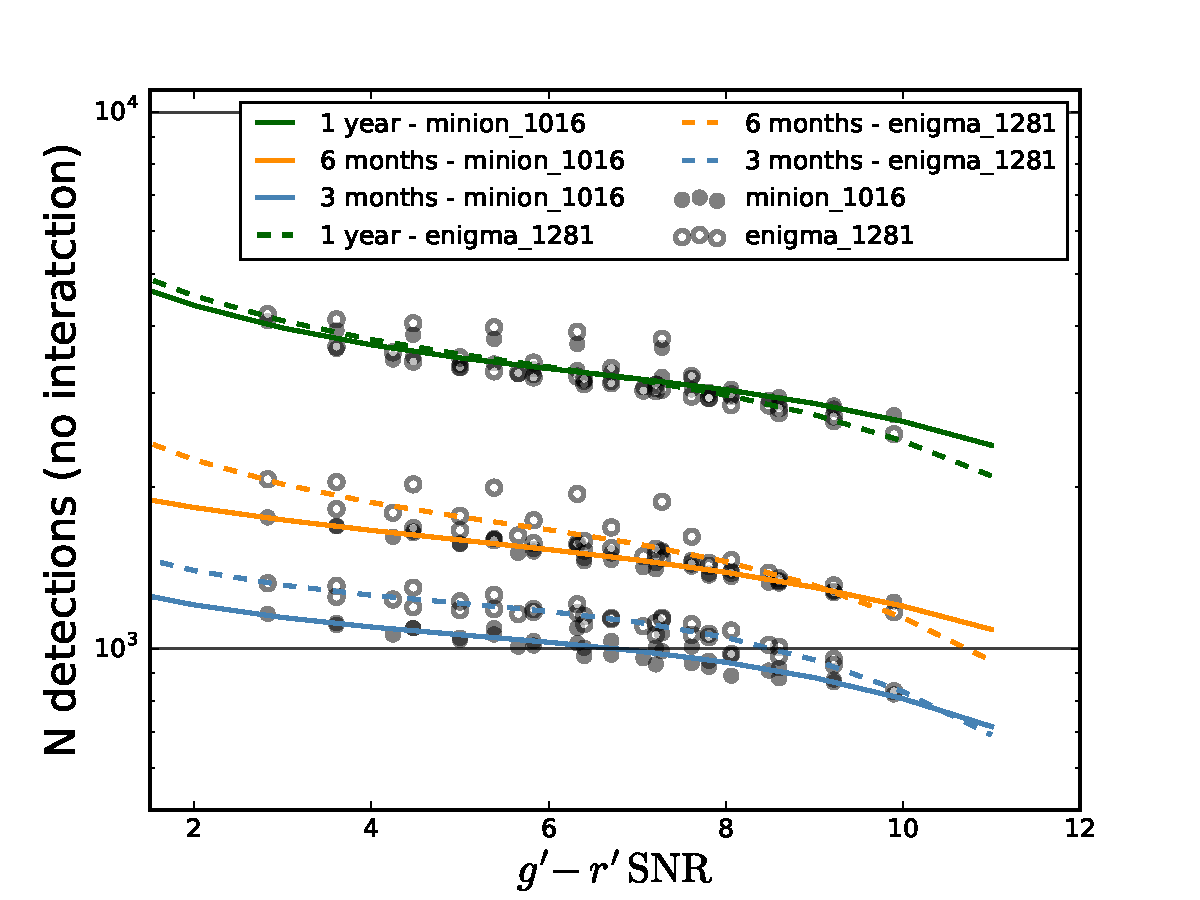
\includegraphics[width=0.6\textwidth]{figs/transients/LSST_Iadetected_wcolor.pdf}
  }
  \caption{
    Normal SN Ia light cure at z=0.5 detected by the \opsimdbref{db:baseCadence} (solid lines) and \opsimdbref{db:NEOswithVisitTriplets} cadence (dashed line) in 3 months, 6 months, and 1 year, that provide color information useful to constrain the progenitor distribution. Line are third-degree polynomial fits.}
  \label{fig:sndetect}
\end{figure}

% ====================================================================
%
 \subsection{Conclusions}

 Here we answer the ten questions posed in
 \autoref{sec:intro:evaluation:caseConclusions}:

 \begin{description}

 \item[Q1:] {\it Does the science case place any constraints on the
 tradeoff between the sky coverage and coadded depth? For example,
 should the sky coverage be maximized (to $\sim$30,000 deg$^2$, as e.g.,
 in Pan-STARRS) or the number of detected galaxies (the current baseline
 but with 18,000 deg$^2$)?}

 \item[A1:] Yes, although this question can be answered with a full simulation that includes a coordinate dependent event rate while the current simulation assumes uniform probability of a transient in the field-of-view and cannot evaluate this trade-off


 \item[Q2:] {\it Does the science case place any constraints on the
 tradeoff between uniformity of sampling and frequency of sampling? For
 example, a rolling cadence can provide enhanced sample rates over a
 part of the survey or the entire survey for a designated time at the
 cost of reduced sample rate the rest of the time (while maintaining the
 nominal total visit counts).}

 \item[A2:] Yes: this science case is sensitive to both. A more sophisticated simulation which also measures the ability to correctly identify the epoch of maximum would be more powerful to answer the question.


 \item[Q3:] {\it Does the science case place any constraints on the
 tradeoff between the single-visit depth and the number of visits
 (especially in the $u$-band where longer exposures would minimize the
 impact of the readout noise)?}

 \item[A3:] Yes, because the diagnostic power depends on both the SNR of each observation and the gap between observations.


 \item[Q4:] {\it Does the science case place any constraints on the
 Galactic plane coverage (spatial coverage, temporal sampling, visits
 per band)?}

 \item[A4:] No.


 \item[Q5:] {\it Does the science case place any constraints on the
 fraction of observing time allocated to each band?}

 \item[A5:] Yes, since it relies on obtaining observations in at least 2 filters.


 \item[Q6:] {\it Does the science case place any constraints on the
 cadence for deep drilling fields?}

 \item[A6:] Yes, although the results have not been analyzed separately for WFD and DD fields.


 \item[Q7:] {\it Assuming two visits per night, would the science case
 benefit if they are obtained in the same band or not?}

 \item[A7:] No. Although  we would benefit greatly from 2 visits in the same filters, and one visit in a different filter to constrain simultaneously shape and color."


 \item[Q8:] {\it Will the case science benefit from a special cadence
 prescription during commissioning or early in the survey, such as:
 acquiring a full 10-year count of visits for a small area (either in
 all the bands or in a  selected set); a greatly enhanced cadence for a
 small area?}

 \item[A8:] A full event rate needs to be included in the simulation to answer this question.


 \item[Q9:] {\it Does the science case place any constraints on the
 sampling of observing conditions (e.g., seeing, dark sky, airmass),
 possibly as a function of band, etc.?}

 \item[A9:] Indirectly, since detection efficiency depends on SNR.


 \item[Q10:] {\it Does the case have science drivers that would require
 real-time exposure time optimization to obtain nearly constant
 single-visit limiting depth?}

 \item[A10:] No.

 \end{description}

 \navigationbar
